\documentclass[a4paper, 12pt]{article}
\usepackage{titlesec}
\usepackage[ngerman]{babel}
\usepackage[a4paper, left=3cm, right=3cm, top=2cm, bottom=2cm]{geometry}
\usepackage{fouriernc}
\usepackage{titlesec}
\usepackage{keystroke}

\newcommand{\makeTitleAndTable}{
    \begin{titlepage}
        \centering
        \vspace*{1.5cm}
        {\Huge Einfacher SPH Flüssigkeitssimulator mit Beschleunigter Nachbarschaftssuche\par}
        \vspace{1cm}
        {\LARGE Thierry Meiers\par}
        {\Large Bachelor Projekt\par}
        \begin{figure}[H]
            \centering
            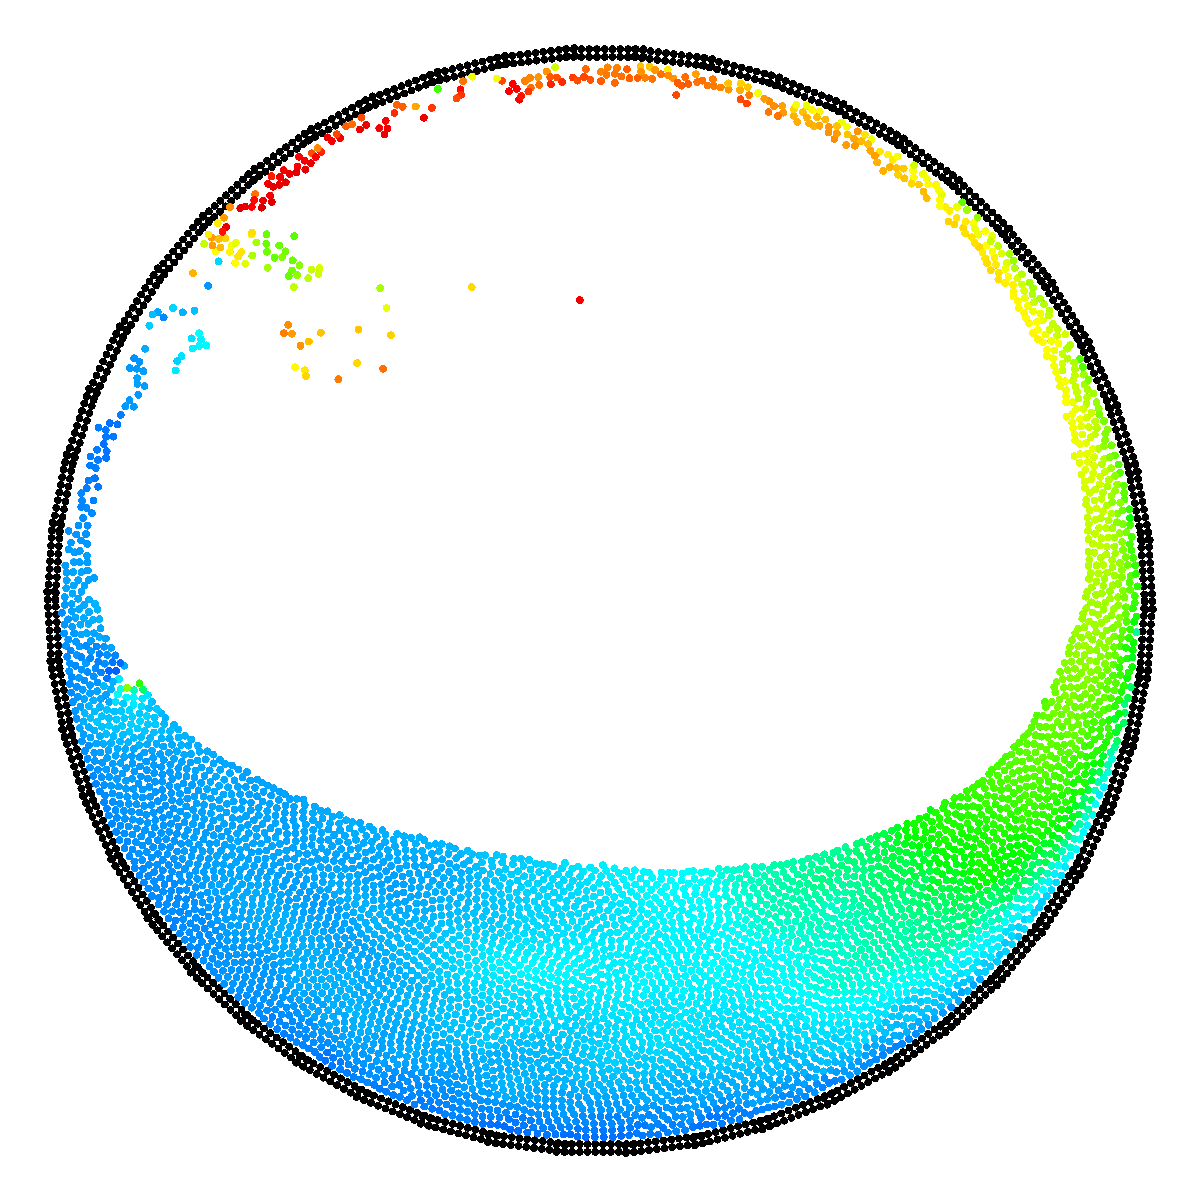
\includegraphics[width=.7\textwidth]{graphics/FirstPage.png}
        \end{figure}
        \vspace{0.5cm}
        {\large Albert-Ludwigs-Universität Freiburg\\Technische Fakultät\\Graphische Datenverarbeitung\par}
        \vfill
        {\large \today \par}
    \end{titlepage}
    \pagenumbering{gobble}
    \tableofcontents
    \clearpage
    \pagenumbering{arabic}
}

\usepackage[
backend=biber,
style=alphabetic,
sorting=ynt
]{biblatex}
\addbibresource{sample.bib} 
\setcounter{tocdepth}{2}

\makeatletter
\def\BState{\State\hskip-\ALG@thistlm}
\makeatother

\begin{document}
\onehalfspacing
\makeTitleAndTable

\section{Einführung}
Fluid Simulationen haben sich zu einem unverzichtbaren Werkzeug in zahlreichen Bereichen unserer Gesellschaft entwickelt. Sie ermöglichen das präzise Simulieren von Flüssigkeiten und Gasen in verschiedenen Umgebungen, wodurch das Verhalten dieser Stoffe und ihre Interaktionen mit der Umgebung untersucht werden können. Aufgrund ihrer Vielseitigkeit kommen Fluid Simulationen in einer großen Bandbreite von Anwendungsgebieten zum Einsatz, darunter die Optimierung von Fahrzeugen und Gebäuden, Wettervorhersagen, medizinische Forschung, die Erzeugung realistischer Effekte in Filmen und Spielen, industrielle Prozesse und Energieerzeugung. Diese Simulationen tragen wesentlich dazu bei, Designs zu verbessern, die Effizienz zu steigern und komplexe Strömungen besser zu verstehen.

Die Allgegenwärtigkeit und Bedeutung dieser Technologie in verschiedenen Branchen wecken das Interesse an dem Thema. Insbesondere die Verbindung von Physik und Informatik weckt zusätzlich persönliche Interessen und ist eine Motivation zur Arbeit an diesem Projekt. Das Hauptziel ist die Implementierung einer Fluid Simulation mit der Smoothed Particle Hydrodynamics (SPH) Methode, um ein tieferes Verständnis für die Komponenten und Mechanismen von SPH zu entwickeln. Um die Performance zu verbessern wird zusätzlich eine beschleunigte Nachbarschaftssuche implementiert. 
Dazu werden zu beginn alle Komponenten von SPH implementiert und auf Korrektheit getestet. Daraufhin werden die einzelnen Komponenten zusammengefügt, woraus sich der Simulationsschritt ergibt. Durch Analysen wird schließlich das Verhalten des Fluiden für verschiedene Einstellungsparameter studiert und interpretiert. Dadurch können die Parameter von SPH richtig gesetzt werden um die Stabilität der Simulation zu optimieren.

In diesem Bericht folgt zuerst eine Motivation. In Abschnitt \ref{Kap:NavierStrokes} werden die Navier-Stokes-Gleichungen vorgestellt. Sie bilden die Grundlage aller Methoden zur Simulation von Fluiden und Gasen. In Abschnitt \ref{Kap:SPH} folgt eine Übersicht aller Komponenten der SPH-Methode, die zur Implementierung der Simulation verwendet wurden. Des weiteren folgt in Abschnitt \ref{Kap:Simulationsschritt} eine Übersicht über den verwendeten Simulationsschritt. Daraufhin wird in Kapitel \ref{Kap:NachbarschaftsSuche} die Funktion der beschleunigten Nachbarschaftssuche erläutert. In Kapitel \ref{Kap:Implementierung} werden einige erwähnenswerte Implementierungen erläutert. Schlussendlich wird in Kapitel \ref{Kap:Alanysen} die Analysen des Simulation vorgestellt.

\section{Navier-Stokes-Gleichungen} \label{Kap:NavierStrokes}
Die Navier-Stokes-Gleichungen sind fundamentale Gleichungen in der Fluidmechanik, die das Verhalten von strömenden Flüssigkeiten und Gasen beschreiben. Sie bilden ein System von nichtlinearen partiellen Differentialgleichungen zweiter Ordnung. Diese basieren auf den Prinzipien der Erhaltung von Masse, Impuls und Energie und modellieren die Bewegung des Fluids, indem sie die Einflüsse von Druck, Viskosität und externen Kräften auf das Strömungsverhalten berücksichtigen \cite{studyflix_navierstokes}.

In ihrer klassischen Form sind sowohl die Impulsgleichung \eqref{equ:Impulsgleichung} als auch die Kontinuitätsgleichung \eqref{equ:Kontinuitätsgleichung} spezifisch für Newtonsche Fluide formuliert. Newtonsche Fluide zeichnen sich durch ein lineares viskoses Fließverhalten aus, bei dem die Viskosität unabhängig von der Schergeschwindigkeit ist.


\subsection{Impulsgleichung}
\begin{equation} \label{equ:Impulsgleichung}
	\rho(\nabla \vec{v} + (\vec{v} \cdot \vec{\nabla})\vec{v}) = - \vec{\nabla}p + \eta \vec{\nabla}^2 \vec{v} + (\lambda + \eta)\vec{\nabla}(\vec{\nabla} \cdot \vec{v}) + \rho \vec{f}
\end{equation}

Gleichung \eqref{equ:Impulsgleichung} beschreibt die Impulserhaltung für komprimierbare Fluide. Diese entspricht dem zweiten Newtonschen Gesetz und kann dementsprechend hergeleitet werden:
\begin{align}
	\vec{F} & =\Delta m \cdot a = \Delta m \cdot \nabla \vec{v} \nonumber                 \\
	\vec{F} & =\rho \cdot \Delta V \cdot \nabla \vec{v} \nonumber                         \\
	\vec{F} & =\rho \cdot \Delta V (\nabla \vec{v} + (\vec{v} \cdot \vec{\nabla})\vec{v})
	\label{equ:Newtonsches_Gesetz}
\end{align}

Die Masse eines Objektes kann durch $m = \rho * V$ bestimmt werden. Die Geschwindigkeitsänderung ergibt sich aus der lokalen zeitlichen Beschleunigung $\nabla \vec{v}$ und der konvektiven Beschleunigung $(\vec{v} \cdot \vec{\nabla})\vec{v}$, also aus der Änderung der Geschwindigkeit aufgrund der Bewegung der Flüssigkeit selbst.

Wir benötigen nun die Kräfte $\vec{F}$. Diese setzen sich aus verschiedenen Kräften zusammen, welche auf einen Fluid wirken. Die Druckkraft \eqref{equ:Druck}, die Reibungskraft \eqref{equ:Reib}, die Kompressionskraft \eqref{equ:Kompress} und die Kräfte, die von außen wirken \eqref{equ:ext}.

\begin{align}
	\vec{F}_{Druck}    & = - \vec{\nabla}p \cdot \Delta V \label{equ:Druck}                                             \\
	\vec{F}_{Reib}     & = \eta \vec{\nabla}^2 \vec{v} \cdot \Delta V \label{equ:Reib}                                  \\
	\vec{F}_{Kompress} & = (\lambda + \eta)\vec{\nabla}(\vec{\nabla} \cdot \vec{v}) \cdot \Delta V \label{equ:Kompress} \\
	\vec{F}_{ext}      & = \rho \vec{f} \cdot \Delta V \label{equ:ext}
\end{align}

\begin{equation} \label{equ:Kraft}
	\vec{F} = \vec{F}_{Druck} + \vec{F}_{Reib} + vec{F}_{Kompress} + \vec{F}_{ext}
\end{equation}

Wir setzen \eqref{equ:Kraft} in die Gleichung \eqref{equ:Newtonsches_Gesetz} ein und erhalten somit:

\[- \vec{\nabla}p \cdot \Delta V\;+\;\eta \vec{\nabla}^2 \vec{v} \cdot \Delta V\;+\;(\lambda + \eta)\vec{\nabla}(\vec{\nabla} \cdot \vec{v}) \cdot \Delta V\;+\;\rho \vec{f} \cdot \Delta V = \rho \cdot \Delta V (\nabla \vec{v} + (\vec{v} \cdot \vec{\nabla})\vec{v})\]

Durch das Dividieren beider Seiten mit $\Delta V$ erhält man schließlich die Gleichung \eqref{equ:Impulsgleichung}.

\[- \vec{\nabla}p + \eta \vec{\nabla}^2 \vec{v} + (\lambda + \eta)\vec{\nabla}(\vec{\nabla} \cdot \vec{v}) + \rho \vec{f} = \rho (\nabla \vec{v} + (\vec{v} \cdot \vec{\nabla})\vec{v})\]

\subsection{Kontinuitätsgleichung}
Des Weiteren folgt die Kontinuitätsgleichung \eqref{equ:Kontinuitätsgleichung}, welche die Erhaltung der Masse innerhalb eines Fluides beschreibt.

\begin{equation} \label{equ:Kontinuitätsgleichung}
	\Delta \rho + \vec{\nabla} \cdot (\rho \vec{v}) = 0
\end{equation}

Sie stellt sicher, dass die zeitliche Änderung der Dichte \(\Delta \rho\) und die Divergenz des Massenflusses \(\vec{\nabla} \cdot (\rho \vec{v})\) sich so ausgleichen, dass die Gesamtmasse konstant bleibt. In einem stationären Strömungsfeld (\(\Delta \rho = 0\)) besagt die Gleichung, dass der Massenzufluss und -abfluss ausgeglichen sein müssen.

\subsection{Nicht komprimierbare Fluide}
Für nicht komprimierbare Fluide vereinfachen sich die Impulsgleichung \eqref{equ:Impulsgleichung} und die Kontinuitätsgleichung \eqref{equ:Kontinuitätsgleichung},

\begin{equation} \label{equ:einfachImpulsgleichung}
	\rho(\nabla \vec{v} + (\vec{v} \cdot \vec{\nabla})\vec{v}) = - \vec{\nabla}p + \eta \vec{\nabla}^2 \vec{v} + \rho \vec{f}
\end{equation}

da \((\lambda + \eta)\vec{\nabla}(\vec{\nabla} \cdot \vec{v}) = 0\) für nicht komprimierbare Fluide und,

\begin{equation} \label{equ:einfachKontinuitätsgleichung}
	\vec{\nabla} \vec{v} = 0
\end{equation}

da \(\Delta \rho = 0\) und \(\vec{\nabla}\rho = 0\)

\section{Smoothed Particle Hydrodynamics} \label{Kap:SPH}
Smoothed Particle Hydrodynamics (SPH) ist eine numerische Methode zur Approximation der Navier-Stokes-Gleichungen. Im Verlauf des Kapitels werden die einzelnen Bestandteile von SPH erläutert und die Verbindung von SPH und den Navier-Stokes-Gleichungen beleuchtet.

Das Konzept von SPH lässt sich allgemein als eine Methode zur Diskretisierung von räumlichen Feldgrößen und räumlichen Differentialoperatoren verstehen. Die zentrale Idee von SPH ist es, Partikel einzusetzen, die Proben von Feldgrößen enthalten und eine Kernel Funktion zu nutzen, um kontinuierliche Felder zu approximieren \cite{huang2024journey}. Ein Partikel besitzt Eigenschaften wie die Masse \( m_i \), die Position \( x_i \), die Geschwindigkeit \( v_i \) und den Druck \( \rho_i \).

\subsection{Kernel Funktion}
Die Kernel Funktion \(W_{ij} = W(x_i - x_j, h)\) ist eine Funktion zur Glättung der Räumlichen Diskretisierung, wobei \(h\) als die Glättungslänge des Kernels bezeichnet wird \cite{10.1111:cgf.14508}. Diese steuert, wie stark der Wert an Position \(x_j\) Einfluss auf den Wert an Position \(x_i\) nimmt. Dabei soll die Kernel Funktion zweifach ableitbar sein und folgende Eigenschaften besitzen \cite: \(\forall x_i, x_j \in \mathds{R}^d, h\in \mathds{R}^+ \rightarrow \int_{\mathds{R}^d}\)
\begin{align}
	W(x_i - x_j', h) dx_j' &= 1 \label{kernelEigenschaft1}\\
	\lim_{h'\rightarrow 0} W(x_i - x_j, h') &= \delta(r) \label{kernelEigenschaft2}\\
	W(x_i - x_j, h) &\geq 0 \label{kernelEigenschaft3}\\
	W(x_i - x_j, h) &= W(-(x_i - x_j), h) \label{kernelEigenschaft4}\\
	W(x_i - x_j, h) &= 0\;:\; |x_i - x_j| \geq h \label{kernelEigenschaft5}
\end{align}
wobei \(\delta(x)\) die Delta-Verteilung ist. 
In diesem Projekt wird die Cubic Spline Kernel Funktion verwendet, wie in \cite{professor_presentation_2024} beschrieben:
\begin{equation*}
	W_{ij} = W(x_j - x_i, h) = \alpha \begin{cases} 
	(2-\frac{\|x_j - x_i\|}{h})^3 - 4(1-\frac{\|x_j - x_i\|}{h})^3 & 0 \leq \frac{\|x_j - x_i\|}{h} \leq 1\\
	(2-\frac{\|x_j - x_i\|}{h})^3 & 1 \leq \frac{\|x_j - x_i\|}{h} \leq 2 \\
	0 & \frac{\|x_j - x_i\|}{h} \geq 2 
	\end{cases}
\end{equation*}

\begin{figure}[H]
	\centering
	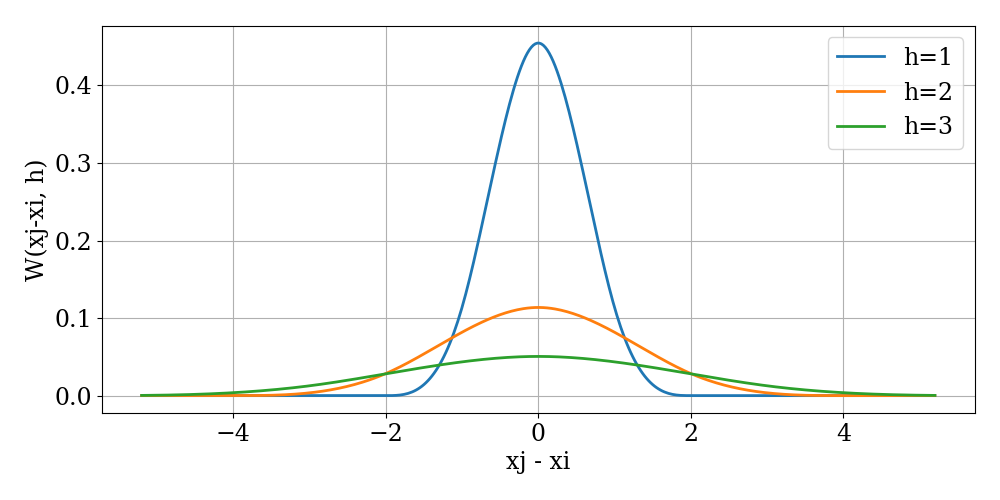
\includegraphics[width=\textwidth]{graphics/KernelPlot.png}
	\caption{Plot der Kernel Funktion für Verschiedene h}
\end{figure}

Dabei ist \(\alpha\) ein Normalisierungsfaktor, der in verschiedenen Dimensionen wie folgt definiert ist:
1D: \(\alpha = \frac{1}{6h}\), 2D: \(\alpha = \frac{5}{14\pi h^2}\), 3D: \(\alpha = \frac{1}{4\pi h^3}\)

\subsection{Kernel Ableitung}
Die Ableitung der Kernel Funktion $W_{ij}$ \cite{professor_presentation_2024} spielt eine entscheidende Rolle bei der Berechnung von Gradienten in der SPH. Sie wird insbesondere zur Berechnung der Druck- und Geschwindigkeitsgradienten verwendet. Die Ableitung der Kernel Funktion $\nabla_i W_{ij}$ bezüglich der Position des Partikels $i$ ist wie folgt definiert:

\begin{equation*}
	\nabla W_{ij} = \nabla W(x_j - x_i, h) = \alpha \frac{x_j - x_i}{\|x_j - x_i\|h} 
	\begin{cases} 
	-3(2-\frac{\|x_j - x_i\|}{h})^2 + 12(1-\frac{\|x_j - x_i\|}{h})^2 & 0 \leq \frac{\|x_j - x_i\|}{h} < 1 \\ 
	-3(2-\frac{\|x_j - x_i\|}{h})^2 & 1 \leq \frac{\|x_j - x_i\|}{h} < 2 \\ 
	0 & \frac{\|x_j - x_i\|}{h} \geq 2 
	\end{cases}
\end{equation*}	

\begin{figure}[H]
	\centering
	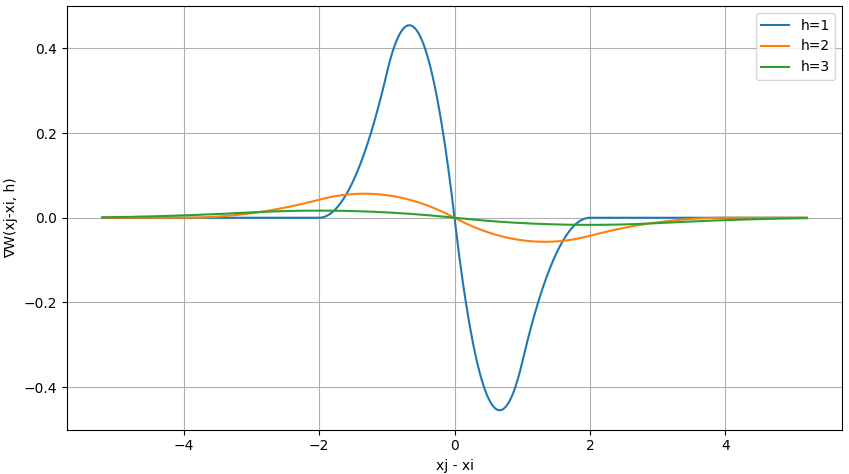
\includegraphics[width=\textwidth]{graphics/KernelDerivPlot.png}
	\caption{Plot der Kernel Ableitung Funktion für verschiedene h}
\end{figure}

Die Kernel Ableitung ist entscheidend, weil sie in mehreren wichtigen Gleichungen verwendet wird, wie z.B. bei der Berechnung der Kontinuitätsgleichung, der Impulsgleichung, insbesondere bei der Berechnung der Druck- und Viskositätsbeschleunigung.

\subsection{Kontinuitätsgleichung}
Die Kontinuitätsgleichung beschreibt die Erhaltung der Masse und wird in der SPH-Methode wie folgt diskretisiert:
\[
\frac{d\rho_i}{dt} = \sum_j m_j (v_i - v_j) \cdot \nabla_i W_{ij}
\]
Dabei ist \(\rho_i\) die Dichte des Partikels \(i\), \(m_j\) die Masse des Partikels \(j\), \(v_i\) und \(v_j\) die Geschwindigkeiten der Partikel \(i\) und \(j\), und \(\nabla_i W_{ij}\) das Gradientenfeld der Kernel Funktion bezüglich des Partikels \(i\).

\subsection{Impulsgleichung}
Die Impulsgleichung beschreibt die Erhaltung des Impulses und wird in der SPH-Methode wie folgt diskretisiert:
\[
\frac{d v_i}{dt} = -\sum_j m_j \left( \frac{p_i}{\rho_i^2} + \frac{p_j}{\rho_j^2} \right) \nabla_i W_{ij} + 2 \nu \sum_j \frac{m_j}{\rho_j} \frac{(v_i - v_j) \times (x_i - x_j)}{(x_i - x_j) \times (x_i - x_j) + 0.01\cdot h^2} \nabla_i W_{ij} + f_i
\]

\subsubsection{Druckbeschleunigung}
Die Beschleunigung aufgrund des Drucks wird durch die folgende Gleichung \cite{monaghan1992smoothed} beschrieben:
\begin{equation} \label{equ:druckBesch}
	a_{druck} = -\sum_j m_j \left( \frac{p_i}{\rho_i^2} + \frac{p_j}{\rho_j^2} \right) \nabla_i W_{ij}
\end{equation}
Dabei sind \( p_i \) und \( p_j \) die Drücke der Partikel \( i \) und \( j \), \(\rho_i \) und \(\rho_j \) die Dichten der Partikel \( i \) und \( j \), und \( \nabla_i W_{ij} \) der Gradient der Kernel Funktion bezüglich des Partikels \( i \).

\subsubsection{Viskositätsbeschleunigung}
Die Beschleunigung aufgrund der Viskosität wird durch die folgende Gleichung \cite{monaghan1992smoothed} beschrieben:
\begin{equation} \label{equ:viskositätBesch}
	a_{viskosität} = 2 \nu \sum_j \frac{m_j}{\rho_j} \frac{(v_i - v_j) \cdot (x_i - x_j)}{(x_i - x_j) \cdot (x_i - x_j) + 0.01\cdot h^2} \nabla_i W_{ij}
\end{equation}
Hier ist \(\nu\) die kinematische Viskosität, \( v_i \) und \( v_j \) sind die Geschwindigkeiten der Partikel \( i \) und \( j \), \( x_i \) und \( x_j \) sind die Positionen der Partikel \( i \) und \( j \), und \(\nabla_i W_{ij}\) ist der Gradient der Kernel Funktion bezüglich des Partikels \( i \).

\subsubsection{Externe Kräfte}
Die externen Kräfte, die auf ein Partikel wirken, werden durch \( f_i \) dargestellt. Dies kann beispielsweise die Gravitation oder andere externe Einflüsse umfassen:
\begin{equation}
	a_{extern} = f_i
\end{equation}
\subsection{Berechnung der Partikeleigenschaften}
\subsubsection{Dichteberechnung}
Die Dichte jedes Partikels \(i\) wird durch die Summe der Massen der benachbarten Partikel \(j\) gewichtet durch die Kernel Funktion berechnet:
\begin{equation} \label{equ:localDichte}
	\rho_i = \sum_j m_j W_{ij}
\end{equation}

\subsubsection{Druckberechnung}
Der Druck \(p_i\) wird häufig durch eine Zustandsgleichung \cite{Adams2007} berechnet, z.B.:
\begin{equation} \label{equ:lokalDruck}
	p_i = k (\frac{\rho_i}{\rho_0} - 1)
\end{equation}
wobei \(k\) die Steifigkeit Konstante ist und \(\rho_0\) die Ruhe-Dichte.

\section{Implementierung} \label{Kap:Implementierung}
Die Implementierung ist zentraler Bestandteil des Projektes. Implementiert wurde in C\# mit Hilfe des Frameworks Monogame. In diesem Kapitel wird die Implementierung von Tests, essenziell für die Korrektheit der Simulation, und die Implementierung Spezieller Hilfsmittel vorgestellt. 

\subsection{Tests}
Das Testen der einzelnen Komponenten des Simulationsschrittes ist essenziell für die Funktionalität und Korrektheit der Simulation. Sie helfen dabei offensichtliche Probleme in der Simulation zu isolieren und zu korrigieren. Allerdings sind ebenfalls nicht offensichtliche Fehler in der Simulation nicht auszuschließen, weshalb die Tests ebenfalls zusätzliche Sicherheit garantieren. Diese werden beim Starten der Simulation gestartet. Dabei wird ein ideales Gitter der Größe  $10 \cdot 10$  mit Partikeln erzeugt. \glqq Ideale\grqq{}, dass alle Partikel den gleichen Abstand h zueinander haben. Auf diesen Partikeln werden schließlich die Tests angewendet. Schlägt ein Test fehl, erscheint eine Nachricht in roter Schrift auf dem Bildschirm. 

Das Fundament aller Berechnungen ist die Nachbarschaftssuche. Ausschließlich bei diesem Test wird ein kleineres ideales Gitter mit $5 \cdot 5$ Partikeln erzeugt.
Die gefundenen Partikel werden in einer Liste Gesammelt. Somit wird gewährleisten dass alle Partikel, die sich im Such-Radius um den mittleren Partikel befinden, gefunden werden. Die Anzahl der Partikel in der Liste muss nach dem Suchen 13 ergeben.

Für die folgenden Tests werden für alle Partikel aus dem größerem Gitter die Nachbarn gesucht und die Komponenten getestet. 
Begonnen wird mit der Kernel Funktion. Eine falsche Gewichtung der Nachbarn in den Berechnungen führt zu falschen Kräften und Bewegungen der Teilchen. Um die Funktionalität der Kernel Funktion zu gewährleisten werden folgende vier Tests \cite{huang2024journey} auf diese angewandt:

\begin{align*}
	\sum_{j} W_{ij} &= \frac{1}{h^2}\\
	W(1, 0) &= \alpha ((2-0)^3 - 4(1-0)^3) = \alpha (8 - 4) = 4\alpha\\
	W(1, 1) &= \alpha ((2-1)^3) = \alpha\\
	W(h, 2) &= 0
\end{align*}

Weiterhin wird die Funktionalität der Kernel Ableitung getestet. Diese ist ein wesentlicher Bestandteil der Gleichungen zum Berechnen der wirkenden Kräfte auf die Partikel. Auf dieser Komponente werden folgende zehn Tests \cite{huang2024journey} angewandt:

\begin{align*}
	\sum_{j} \Delta W_{ij} &= (0, 0)\\
	\Delta W(h, 0) &= (0, 0)\\
	\Delta W(h, (0, 0) - (\pm h, 0)) &= (\frac{3\alpha}{h}, 0)\\
	\Delta W(h, (0, 0) - (0, \pm h)) &= (0, \frac{3\alpha}{h})\\
	\Delta W(h, (0, 0) - (h, h)) = \Delta W(h, (0, 0) - (- h, - h))&= (-\frac{9\sqrt{2} - 12}{h} \alpha,-\frac{9\sqrt{2} - 12}{h} \alpha)\\
	\Delta W(h, (0, 0) - (h, -h)) = \Delta W(h, (0, 0) - (-h, h)) &= (-\frac{9\sqrt{2} - 12}{h} \alpha,\frac{9\sqrt{2} - 12}{h} \alpha)
\end{align*}

Ebenfalls werden die Funktionen zum Berechnen lokaler Werte getestet. Da die Partikel sich beim Test in einem idealem Gitter befinden, ergibt die Berechnung der lokalen Dichte die Ruhedichte $\rho_0$.
\[\rho_i = \sum_{j} m_j W_{i, j} = m \sum_{j} W_{i, j} = \frac{m}{h^2} = \rho_0\]
Daraus folgt ebenfalls dass die Funktion des lokalen Drucks 0 ergibt:
\[p_i = k(\frac{\rho_0}{\rho_0} - 1) = k(1 - 1) = 0\]

\subsection{Tools}
Die Simulation verfügt über einige implementierte Tools zur Steuerung der Simulation. Durch das Drücken der Taste \keys{H} öffnet sich eine Liste von Aktionen zum Steuern der Simulation. Einige der wichtigsten Aktionen werden in diesem Unterkapitel vorgestellt. 

Die Simulation verfügt über mehrere verschiedene \glqq Szenarios\grqq{}. Ein \glqq Szenarios\grqq{} bedeutet hier, eine Box oder eine andere geometrische Form, welche eine Barriere für die zu simulierende Flüssigkeit bildet. Diese können mit der Taste \keys{V} gewechselt werden. Durch das Wechseln der Szene oder Drücken der Taste \keys{del} werden alle Partikel der Szene gelöscht. 

Ebenfalls können zu Zwecken der Simulation Partikel mit Hilfe der Maus in der jeweiligen Szene platziert werden. Dazu wird mit der Taste \keys{Q} die Form einer Box, eines Kreises oder eines einzelnes Partikels
ausgewählt. Im Falle der Box und des Kreises können die Höhe und Breite verändert werden. \keys{W}, \keys{S} vergrößern bzs. verkleinern die Höhe, \keys{D}, \keys{A}vergrößern bzs. verkleinern die Breite. Platziert werden die Partikel durch ein Linksklick.

Im Sinne der Analyse können durch das Drücken der Taste \keys{F2} Daten gesammelt werden und durch das Drücken von \keys{F1} gespeichert werden. Zusätzlich wird durch drücken der Taste \keys{F12} ein Screenshot aufgenommen. Gespeichert werden alle Dateien im Dokumentenordner des Benutzers.

\subsection{Parallelisierung des Simulationsschrittes}
Die ersten beiden Schleifen des Simulationsschrittes (siehe Kapitel \ref{Kap:Simulationsschritt}) wurden mit Hilfe der Funktion Parallel.ForEach() implementiert. Diese Funktion ermöglicht es, die einzelnen Prozesse auf verschiedene Threads der CPU aufzuteilen. Dabei wartet die Funktion automatisch, bis alle Threads ihre Aufgaben abgeschlossen haben, bevor die Verarbeitung im sequentiellen Code fortgesetzt wird. Da beide Schleifen auf Hashtabellen zugreifen werden diese Zugriffe gesperrt um Wettlaufsituation zu verhindern.  

\subsection{Färbung der Geschwindigkeit}
Die Färbung der Partikel basierend auf dem CFL-Kriterium stellt eine wichtige Funktion der Simulation dar, um die Stabilität der Simulation visuell zu analysieren. Um die Stabilität der Simulation darzustellen, wird eine Farbcodierung verwendet, bei der die Farbe proportional zum CFL-Wert variiert.
Der CFL-Wert wird berechnet als $\text{CFL} = \frac{v \Delta t}{h}$, wobei \(v\) die Geschwindigkeit des Partikels, \(\Delta t\) der Zeitschritt und \(h\) die Partikelgröße ist.
Die Partikel werden proportional zum CFL-Wert im Farbspektrum von Blau bis Rot eingefärbt. Durch diesen Farbverlauf wird eine intuitive visuelle Darstellung der Stabilität im gesamten Simulationsraum ermöglicht.
 
\subsection{Behandlung von Grenzen}
Die Simulation findet in einem eingeschränktem Raum satt. Dieser Raum wird mithilfe einer Grenze aus Grenzpartikeln gebildet. Die Breite der Grenze beträgt zwei Partikel. Dadurch füllen die Grenzpartikel alle freien Nachbarstellen eines Flüssigkeitspartikels. Die Position der  Grenzpartikel bleibt im Verlauf der Simulation konstant. 

In der Implementierung werden bei der Berechnung der Beschleunigungen die Flüssigkeitspartikel von Grenzpartikeln differenziert. Die implementierte Gleichung zur Druckbeschleunigung \eqref{equ:druckBesch} lautet: $\forall j_f \in \text{Flüssigkeitspartikel}, \forall j_b \in \text{Grenzpartikel}$ 

\begin{equation} \label{equ:druckBeschGrenze}
	a_{druck} = -\sum_{j_f} m_{j_f} \left( \frac{p_i}{\rho_i^2} + \frac{p_{j_f}}{\rho_{j_f}^2} \right) \nabla_i W_{i{j_f}} -\sum_{j_b} p_i 2\frac{m_i}{\rho_i^2} \nabla_i W_{i{j_b}}
\end{equation}

Zusätzlich wird bei der Viskositätsbeschleunigung \eqref{equ:viskositätBesch} der Einfluss der Grenze verringert, indem die Viskosität für Grenzpartikel verringert wird:

\begin{align}
	a_{viskosität} &= 2 \nu \sum_{j_f} \frac{m_{j_f}}{\rho_{j_f}} \frac{(v_i - v_{j_f}) \cdot (x_i - x_{j_f})}{(x_i - x_{j_f}) \cdot (x_i - x_{j_f}) + 0.01\cdot h^2} \nabla_i W_{i{j_f}} \nonumber \\
	&+ \nu \sum_{j_b} \frac{m_{j_b}}{\rho_{j_b}} \frac{(v_i - v_{j_b}) \cdot (x_i - x_{j_b})}{(x_i - x_{j_b}) \cdot (x_i - x_{j_b}) + 0.01\cdot h^2} \nabla_i W_{i{j_b}} \label{equ:viskositätBeschGrenze}
\end{align}

\section{Nachbarschaftssuche} \label{Kap:NachbarschaftsSuche}
Die Nachbarschaftssuche ist das Fundament der Simulation. Diese erlaubt das Ermitteln der Nachbarpartikel in einem festen Radius um eine Position zum Berechnen lokaler Werte. Ein naiver Ansatz wäre, für alle Partikel den Abstand zur Position zu ermitteln und zu prüfen, ob sich diese im Radius befinden. Diese Methode weist jedoch eine quadratische Laufzeitkomplexität auf, da für jedes Partikel der Abstand zu allen anderen Partikeln berechnet werden muss. Dies führt zu einer Laufzeit von $O(n^2)$, wobei $n$ die Anzahl der Partikel ist. Bei einer großen Partikelanzahl wird dieser Ansatz daher ineffizient und rechenintensiv.

Für das Projekt wurde dementsprechend das Räumliche Hashing verwendet. Dabei handelt es sich um eine Datenstruktur die den Raum in einzelne Blöcke unterteilt. Beim ermitteln von Nachbarpartikel müssen dadurch nicht mehr alle Partikel geprüft werden sondern nur diese, die sich in dem selbem Block oder Nachbarblock befinden. Dies führt zu einer effizienteren und weniger rechenintensiven Methode zum Bestimmen der Nachbarn.

\subsection{Einfügen von Partikeln}
Um ein Partikel in die Datenstruktur einzufügen wird als erstes ein Hashwert bezüglich der Position errechnet. Dazu wird der Positionsvektor durch die Blockgröße geteilt und das Ergebnis abgerundet.
\begin{algorithm}[H]
	\caption{Hash Funktion}
	\begin{algorithmic}[1]
		\Require Vector $\mathbf{v} = (v_x, v_y)$, scalar $\text{CellSize}$
		\Ensure Hashed vector $\mathbf{h} = (h_x, h_y)$
		\State $\mathbf{h} \leftarrow \frac{\mathbf{v}}{\text{CellSize}}$
		\State $\mathbf{h} \leftarrow \lfloor \mathbf{h} \rfloor$
		\Return $\mathbf{h}$
	\end{algorithmic}
\end{algorithm}

Schließlich wird der Partikel in eine Liste innerhalb der Hashtabelle eingefügt. Das Löschen eines Partikels aus der Datenstruktur funktioniert analog.

\subsection{Updaten der Partikel Positionen}
Wurden die Positionen der Partikel im Simulationsschritt aktualisiert, müssen ebenfalls die Einträge in der Hashtabelle Aktualisiert werden. Dazu werden die Partikel vor dem Aktualisieren der Position aus der Datenstruktur entfernt und nach der Aktualisierung wieder eingefügt. 

\subsection{Ermitteln von Nachbarn}
Das ermitteln von Nachbar Partikeln ist das Fundament des Simulationsschrittes. Zu erst werden die Blöcke, welche Teil des Radiuses sind und somit durchsucht werden müssen, ermittelt. Des Weiteren werden die Partikel in den Blöcke überprüft, ob sich diese in dem Radius um die Position befinden.
\begin{algorithm}[H]
    \caption{Partikel im Radius}
    \begin{algorithmic}[1]
		\Require Position $\mathbf{p}$, Radius $r$
        \Ensure Liste der Partikel im Radius: $\text{partikelImRadius}$
        \State $startX \leftarrow \lfloor (\mathbf{p}_x - r) / \text{CellSize} \rfloor$
        \State $endX \leftarrow \lceil (\mathbf{p}_x + r) / \text{CellSize} \rceil$
        \State $startY \leftarrow \lfloor (\mathbf{p}_y - r) / \text{CellSize} \rfloor$
        \State $endY \leftarrow \lceil (\mathbf{p}_y + r) / \text{CellSize} \rceil$
        \For{($x \leftarrow startX$ \textbf{to} $endX$)}
            \For{($y \leftarrow startY$ \textbf{to} $endY$)}
                \If{($(x , y)$ existiert in $\text{Hashtabelle}$)}
                    \ForAll{(Partikel in \text{Hashtabelle}[hash])}
                        \If{($\text{Distance}(Partikel.\text{Position}, \mathbf{p}) \leq r$)}
                            \State $\text{partikelImRadius}.\text{add}(q)$
                        \EndIf
                    \EndFor
                \EndIf
            \EndFor
        \EndFor
        \Return $\text{partikelImRadius}$
    \end{algorithmic}
\end{algorithm}
Dies erlaubt es die Anzahl an Partikeln welche überprüft werden müssen zu beschränken und die Laufzeit zu verringern. 

\section{Simulationsschritt} \label{Kap:Simulationsschritt}
Der Simulationsschritt ist in der SPH Simulation von Zentraler Bedeutung. Dort werden alle nötigen Beschleunigungen ermittelt, die zum simulieren eines Fluides mithilfe von Partikeln, nötig sind. In diesem Projekt wurde die Methode in 3 Schleifen unterteilt wobei die erste als einzige alle Partikel berücksichtigt. In den Restlichen Schleifen werden nur Partikel welche das Fluid bilden beachtet und Partikel zum Simulieren der Grenze Ignoriert. Eigenschaften wie die Partikelgröße und die Ruhedichte der Flüssigkeit werden vor dem Starten der Simulation festgelegt. Aus diesen wird eine Masse für die Partikel ermittelt, welche im Laufe der Simulation konstant bleibt. Eigenschaften wie die Position, Geschwindigkeit, lokale Dichte und lokaler Druck werden im Partikel gespeichert. Die Nachbarn der einzelnen Partikel als auch alle berechneten Beschleunigungen werden in Hashtabellen gespeichert damit diese über alle schleifen zugänglich sind.

\begin{algorithm}[H]
	\caption{Simulationsschritt}
	\begin{algorithmic}[1]
	\State \textbf{Parallel for each} particle \textbf{in} particles
	\State \quad $\text{FindNeighbors()}$
	\State \quad $\text{ComputeLocalDensity()}$ \hfill \text{verwendete Gleichung \eqref{equ:localDichte}}
	\State \quad $\text{max(ComputeLocalPressure(), 0)}$ \hfill \text{verwendete Gleichung \eqref{equ:lokalDruck}}
	\vspace{1em}
	\State \textbf{Parallel for each} particle \textbf{in} noBoundaryParticles
	\State \quad $\text{GetViscosityAcceleration}()$ \hfill \text{verwendete Gleichung \eqref{equ:viskositätBeschGrenze}}
	\State \quad $\text{GetPressureAcceleration}()$ \hfill \text{verwendete Gleichung \eqref{equ:druckBeschGrenze}}
	\vspace{1em}
	\State \textbf{For each} particle \textbf{in} noBoundaryparticles
	\State \quad $\text{acceleration} = \text{viscosityAcceleration} + \text{pressureAcceleration} + \text{gravitation}$
	\State \quad $\text{particle.Velocity} += \text{timeSteps}\;\cdot\;\text{acceleration}$
	\State \quad $\text{particle.Position} += \text{timeSteps}\;\cdot\;\text{particle.Velocity}$
	\end{algorithmic}
	\end{algorithm}

In der ersten Schleife werden die lokalen Eigenschaften ermittelt. Dazu müssen die Nachbarpartikel in einem Radius $2 \cdot \text{Partikelgröße}$ um die Partikel ermittelt werden. Mithilfe der Nachbarn wird die lokale Dichte und der lokale Druck jedes Partikels bestimmt. Diese werden für die Berechnungen der nächsten Schleife benötigt. In dieser werden für alle Partikel die das Fluid bilden, die Viskosität- und Druckbeschleunigungen berechnet. Anhand dieser Beschleunigungen werden die Positionen der Partikel in der letzten schleife aktualisiert. 

\section{Analysen} \label{Kap:Alanysen}
Zuletzt werden die gesammelten Daten von Experimenten visualisiert und vorgestellt. Die Experimente befassen sich mit Schwerpunkten der Simulation. Das erste Experiment beobachtet die Auswirkung der Einstellungsparameter auf die Stabilität um das Verhalten des Fluiden. Dazu wird eine Wassersäule simuliert und das Verhalten der Dichte aller Partikel zu analysieren. Da der Druck innerhalb eines Fluiden Abhängig der Gravitation, Fluid Höhe und Fluid Dichte ist, reicht es hier eine schmale Säule für das Experiment zu nutzen. 
Zunächst wird der Einfluss der beschleunigten Nachbarschaftssuche auf die Performance der Simulation betrachtet. Hierfür wird die Zeit um einen Simulationsschritt zu durchlaufen (Simulationsschrittzeit) beobachtet. Dabei wird die Anzahl an Partikeln kontinuierlich erhöht und in Relation zur Simulationsschrittzeit gesetzt. Dieses Vorgehen wird auf beide Methoden der Nachbarschaftssuche angewandt.
Analog dazu wird ebenfalls betrachtet, wie sich die Performance verhält für eine sequentielle- und parallele Prozessverarbeitung.

\subsection{Säulenexperiment}

In dem durchgeführten Säulenexperiment wurden die Auswirkungen der Steifigkeit \(k\), der Viskosität \(\nu\) und des Zeitschritts \(\Delta t\) auf die lokalen Dichten aller Partikel untersucht. Hierbei wurde in jedem Simulationsschritt der Mittelwert der lokalen Dichten aller Partikel ermittelt und im Verhältnis zu den Simulationsschritten bzw. der Zeit dargestellt. Die Dichten werden in den Grafiken als relativer Dichtefehler angezeigt, der die prozentuale Abweichung von der Ruhedichte angibt. Der relative Dichtefehler dient als Maß für die numerische Kompressibilität des Fluids; ein optimaler Wert wäre ein relativer Dichtefehler von Null. In der Praxis ist dies jedoch schwer zu erreichen, insbesondere bei numerischen Simulationen. Ziel ist es daher, ein Verständnis für die Beziehung zwischen den Parametern und dem Verhalten des Fluids zu entwickeln.

\subsubsection{Steifigkeit k}
\begin{figure}[H]
	\centering
	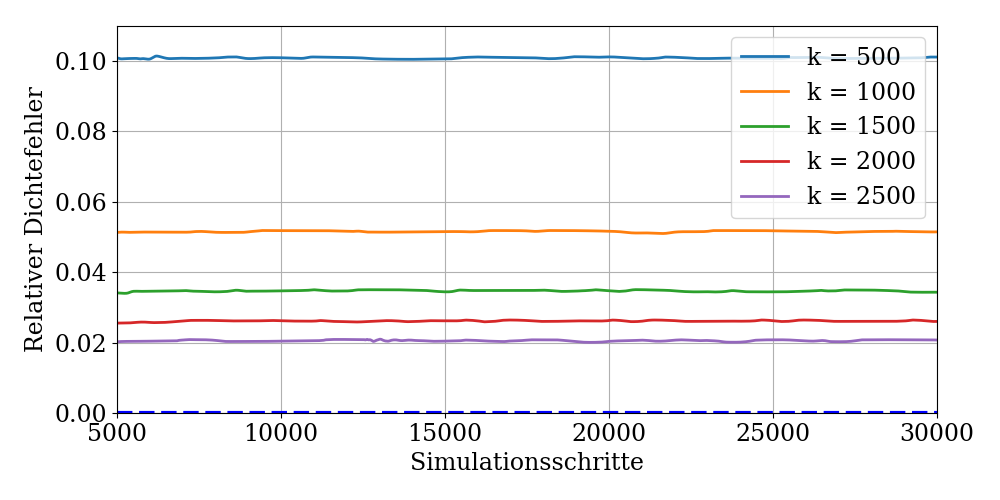
\includegraphics[width=.85\textwidth]{graphics/Steifigkeit.png}	
	\caption{Säulenexperiment mit Verschiedener Steifigkeit k}
	\label{Säulenexperiment_k}
\end{figure}

Der wichtigste Parameter in diesem Zusammenhang ist der Steifigkeitsparameter \(k\). Dieser skaliert die Berechnung der lokalen Dichte \eqref{equ:localDichte} und hat einen direkten Einfluss auf die Druckbeschleunigungen \eqref{equ:druckBesch} sowie die Kompressibilität des Fluids. In Abbildung \ref{Säulenexperiment_k} wurde das Säulenexperiment mit verschiedenen Werten für \(k\) simuliert. Um die Visualisierung anschaulicher zu gestalten, wurde für dieses Experiment eine hohe Viskosität gewählt, wodurch Schwankungen des Dichtefehlers minimiert werden, was zu einem konstanten Wert führt. Auffällig ist, dass die lokale Dichte konstant bleibt und sich der Dichtefehler mit steigendem \(k\) verringert. Die lokale Dichte konvergiert dabei in Richtung der Ruhedichte. Daraus lässt sich schließen, dass eine höhere Steifigkeit \(k\) die numerische Kompressibilität des Fluids reduziert und somit die Simulation stabiler und präziser wird.

\subsubsection{Viskosität v}
\begin{figure}[H]
	\centering
	\includegraphics[width=.85\textwidth]{graphics/Viskosität.png}	
	\caption{Säulenexperiment mit Verschiedener Viskosität v}
	\label{Säulenexperiment_v}
\end{figure}

Im zweiten Säulenexperiment wurde die Viskosität \(\nu\) variiert. Diese beeinflusst, wie stark ein Partikel von seinen Nachbarn gedämpft wird. Abbildung \ref{Säulenexperiment_v} zeigt, wie die Viskosität die Schwankungen der lokalen Dichte dämpft. Dies wird durch eine Verringerung der Amplitude der Schwankungen deutlich. Je höher die Viskosität, desto stärker dämpfen sich die Partikel gegenseitig, was zu einer schnelleren Anpassung des Fluids an Gleichgewichtszuständen führt. Es ist jedoch wichtig zu beachten, dass eine zu hohe Viskosität das physikalische Verhalten des Fluids verfälschen könnte, indem das Fluid zu zähflüssig erscheint.

\subsubsection{Zeitschritten $\Delta$ t}
\begin{figure}[H]
	\centering
	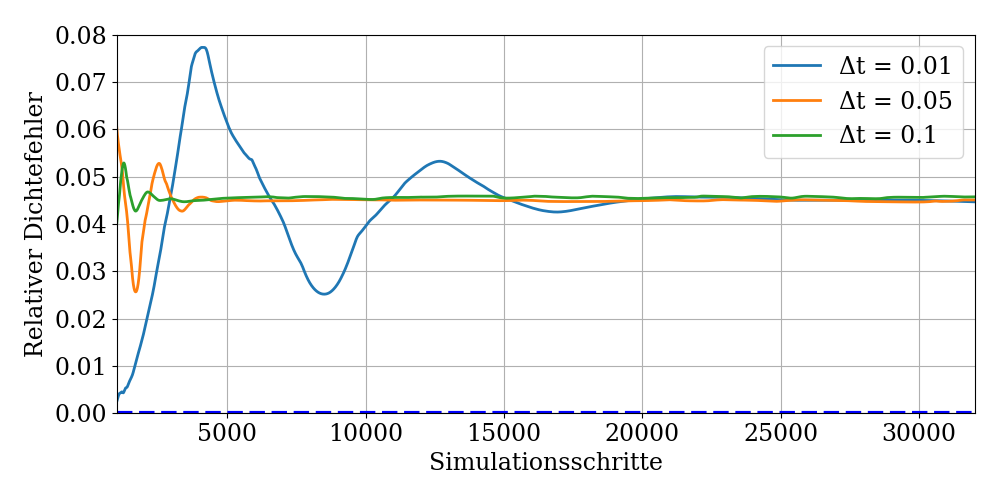
\includegraphics[width=.85\textwidth]{graphics/Zeitschritt.png}	
	\label{Säulenexperiment_t}
	\caption{Säulenexperiment mit Verschiedenen Zeitschritten $\Delta$ t}
\end{figure}

Der letzte untersuchte Parameter ist der Zeitschritt \(\Delta t\). Dieser skaliert die auf die Partikel wirkende Beschleunigung und damit auch die Bewegung der Partikel. In Abbildung \ref{Säulenexperiment_t} ist zu erkennen, dass kleinere Zeitschritte \(\Delta t\) zu einer Vergrößerung der Amplitude und einer Verkleinerung der Frequenz der Dichteschwankungen führen. Die verringerte Frequenz ist darauf zurückzuführen, dass die Bewegungsdistanz der Partikel bei kleineren Zeitschritten innerhalb eines Simulationsschritts reduziert wird. Die größere Amplitude rührt daher, dass bei kleineren \(\Delta t\) auch die Beschleunigungen geringer ausfallen, was dazu führt, dass die Partikel mehrere Simulationsschritte benötigen, bis die Beschleunigungen ihre volle Wirkung entfalten. Es sollte jedoch betont werden, dass ein zu großer Zeitschritt die Simulation instabil machen kann, da wichtige physikalische Prozesse möglicherweise nicht richtig aufgelöst werden. Andererseits können zu kleine Zeitschritte die Rechenzeit erheblich verlängern, ohne einen proportionalen Nutzen in der Genauigkeit zu bringen.

\subsection{Nachbarschaftssuche}

Wie in Kapitel \ref{Kap:NachbarschaftsSuche} erläutert, ist die Nachbarschaftssuche das Fundament. Alle Berechnungen für die Simulation von Fluiden benötigen die Nachbarpartikel. Daher werden diese wie in Kapitel \ref{Kap:Implementierung} beschrieben, für alle Partikel in jedem Simulationsschritt ermittelt. Dabei ist eine effiziente Nachbarschaftssuche von großem Vorteil. Eine schnellere Suche ermöglicht eine weniger rechenintensive Simulation bei einer höheren Anzahl an Partikeln. In dieser Analyse wird geprüft, ob die Benutzung der Räumlichen Datenstruktur die Performance der Simulation, im Vergleich zur Quadratischen suche, positiv beeinflusst wird. Dazu werden während der Simulation kontinuierlich neue Partikel erzeugt. Dabei wird die Simulationsschrittzeit gemessen und in Verhältnis zur Anzahl an Partikeln dargestellt.

\begin{figure}[H]
	\centering
	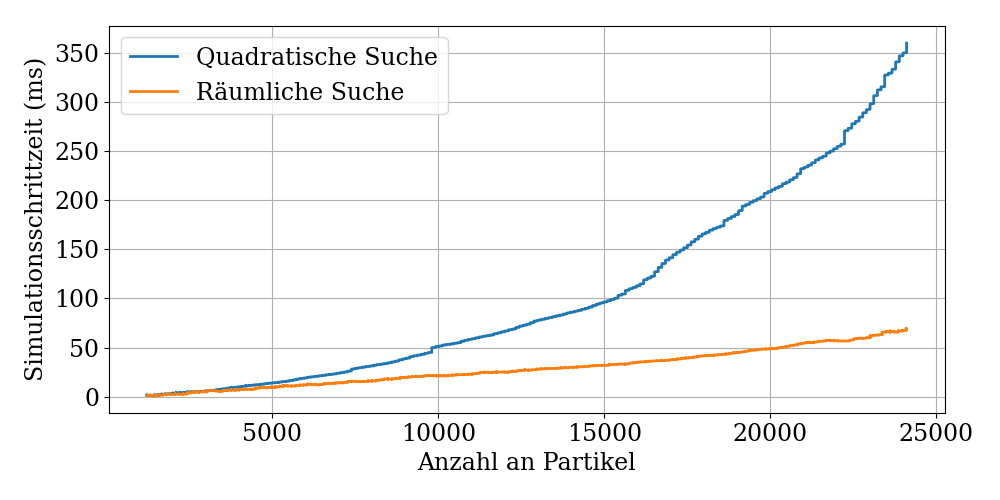
\includegraphics[width=.85\textwidth]{graphics/Nachbarschafts-Suche.png}
	\caption{Nachbarschaftssuche mit Paralleler Prozessverarbeitung}
	\label{NachbarschaftsSuche}
\end{figure}

Wie erwartet steigert sich die Simulationsschrittzeit für die Quadratische Suche, bei erhöhen der Partikel Anzahl, Exponentiell, wobei sich die Simulationsschrittzeit bei der Räumlichen Datenstruktur linear erhöht. Die Räumliche Datenstruktur erlaubt es eine eine erhebliche höhere Anzahl an Partikeln simulieren zu können bei linearem Wachstum des Rechenaufwandes.  

\subsection{Prozessverarbeitung}
Die Parallelisierung des Simulationsschrittes (siehe Kapitel \ref{Kap:Simulationsschritt}) trägt ebenfalls zu einer Verringerung der Simulationsschrittzeit bei. Bei dieser Analyse wird wie zuvor, die Anzahl an Partikeln kontinuierlich erhöht und die Simulationsschrittzeit gemessen. Dies wird dann mithilfe eines sequentiellen Simulationsschrittes und mit einem parallelen Simulationsschritt simuliert.

\begin{figure}[H]
	\centering
	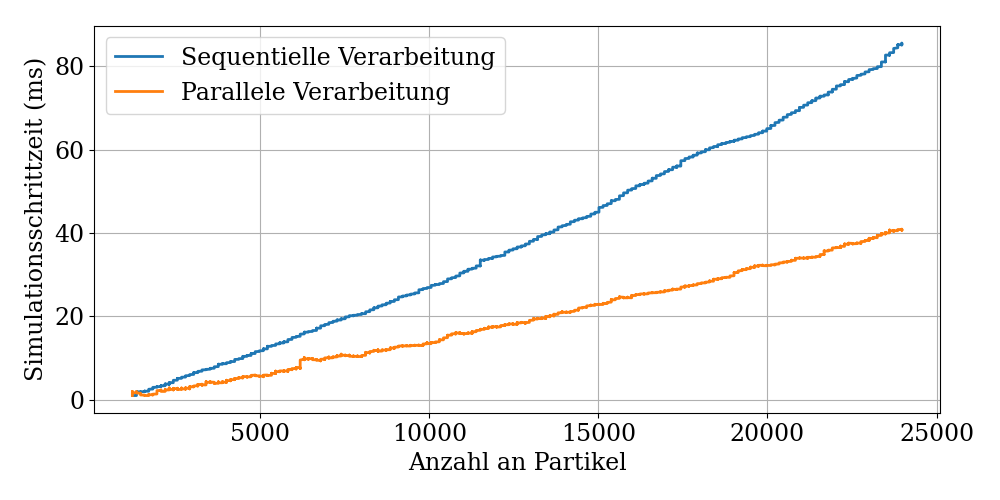
\includegraphics[width=.85\textwidth]{graphics/Prozessverarbeitung.png}
	\caption{Prozessverarbeitung mit beschleunigter Nachbarschaftssuche}
	\label{Prozessverarbeitung}
\end{figure}

Die Ergebnisse (siehe Abbildung \ref{Prozessverarbeitung}) zeigen eine klare Verkürzung der Simulationsschrittzeit bei einer parallelen Prozessverarbeitung. Bei diesen Daten wird die Simulationsschrittzeit bei paralleler Verarbeitung halbiert. Dabei gilt jedoch zu beachten, dass dieser Trend je nach CPU abweichen kann.  

\section{Schlussfolgerung}
Das Ziel dieses Projekts war, eine grundlegende SPH-Simulation (Smoothed Particle Hydrodynamics) zu implementieren, ein vertieftes Verständnis für die SPH-Methode zu entwickeln und die Auswirkungen der Einstellungsparameter auf das Fluidverhalten zu analysieren. SPH erwies sich als eine leistungsfähige und zugleich einfache Methode zur Simulation von Fluiden. Im Rahmen des Projekts wurde ein einfacher SPH-Simulator erfolgreich implementiert. Durch die Integration einer beschleunigten Nachbarschaftssuche und paralleler Verarbeitung konnte eine stabilere und flüssigere Simulation mit einer größeren Anzahl von Partikeln erreicht werden.

Das Projekt trug maßgeblich dazu bei, ein tieferes Verständnis für die zugrunde liegenden Prozesse in SPH zu entwickeln und zu erkennen, wie komplexe Strömungen realistisch simuliert werden können. Die Analyse und Interpretation der experimentellen Ergebnisse ermöglichte es, die Einflüsse der Parameter auf das Fluidverhalten besser zu verstehen und deren Wechselwirkungen zu identifizieren. Dadurch konnte eine stabile Simulation durch gezielte Anpassung der Parameter gewährleistet werden.

Abbildung \ref{exampleSimulation} zeigt den Ablauf des Verhalten eines Fluiden, welcher mit dem SPH-Simulator simuliert wurde. Die Flüssigkeit verhält sich stabil und realistisch, ohne unerwünschte Artefakte oder Instabilitäten. Die Anpassungen führten zu einer präziseren und natürlicheren Darstellung der Fluiddynamik.

\begin{figure}[H]
	\centering
	\subfigure[]{
		\centering
		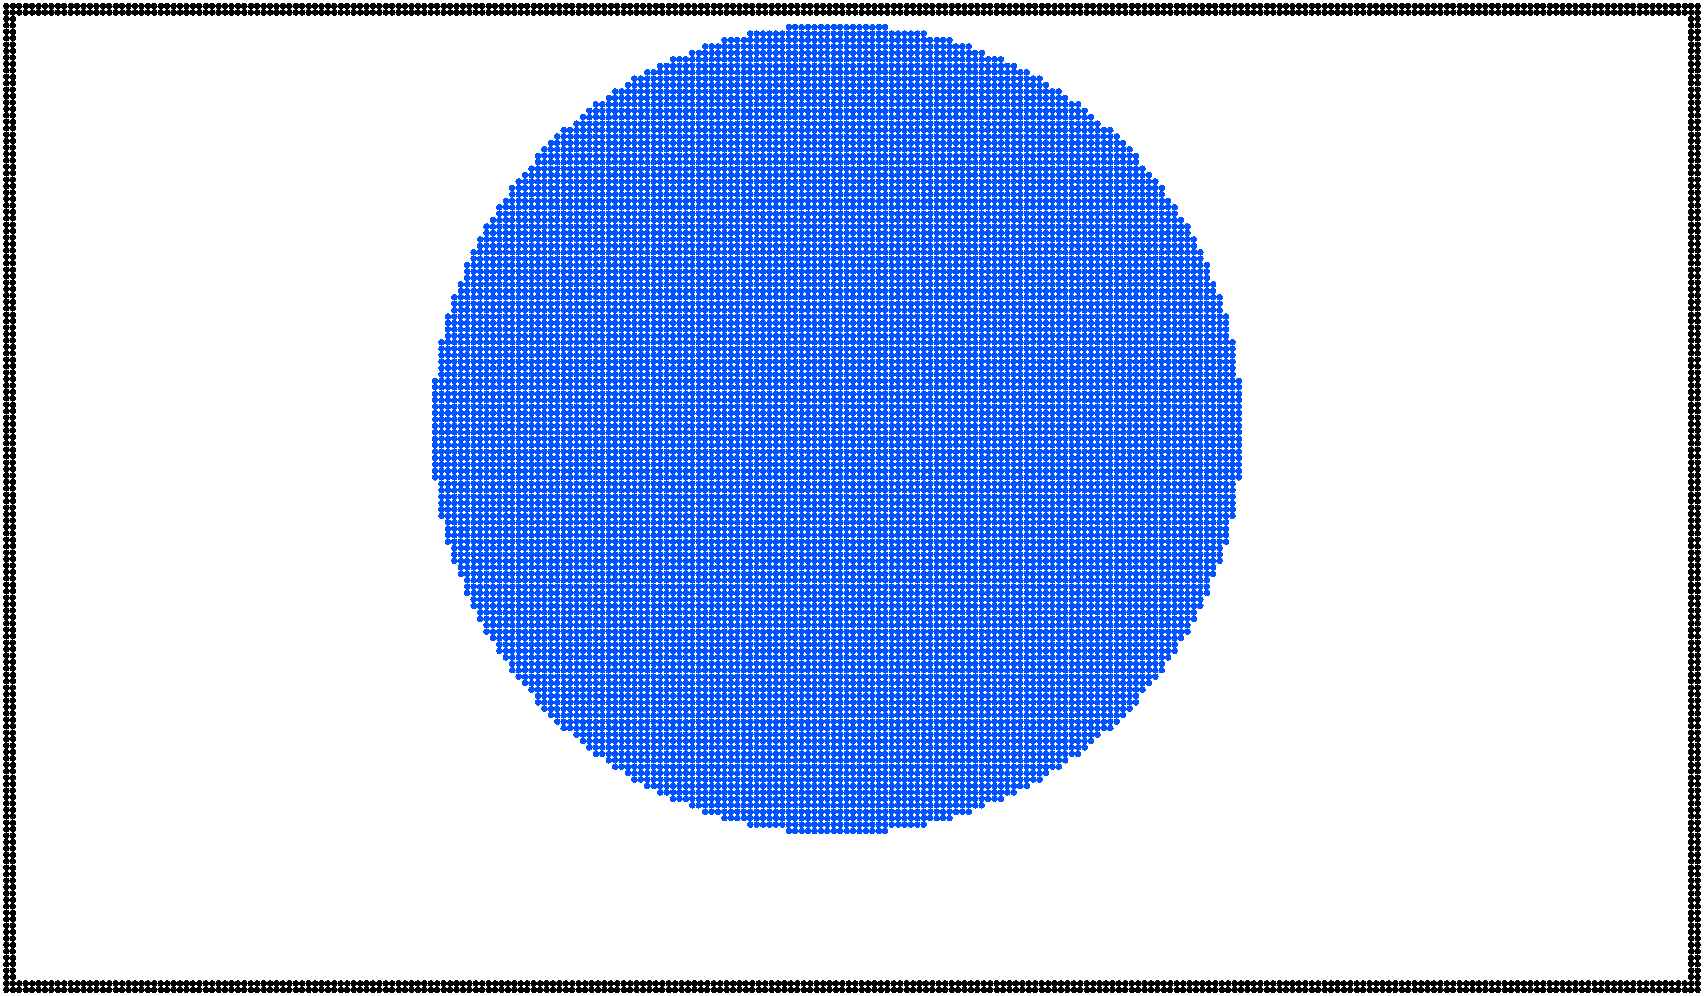
\includegraphics[width=.45\textwidth]{graphics/sim1.png}
	}	
	\subfigure[]{
		\centering
		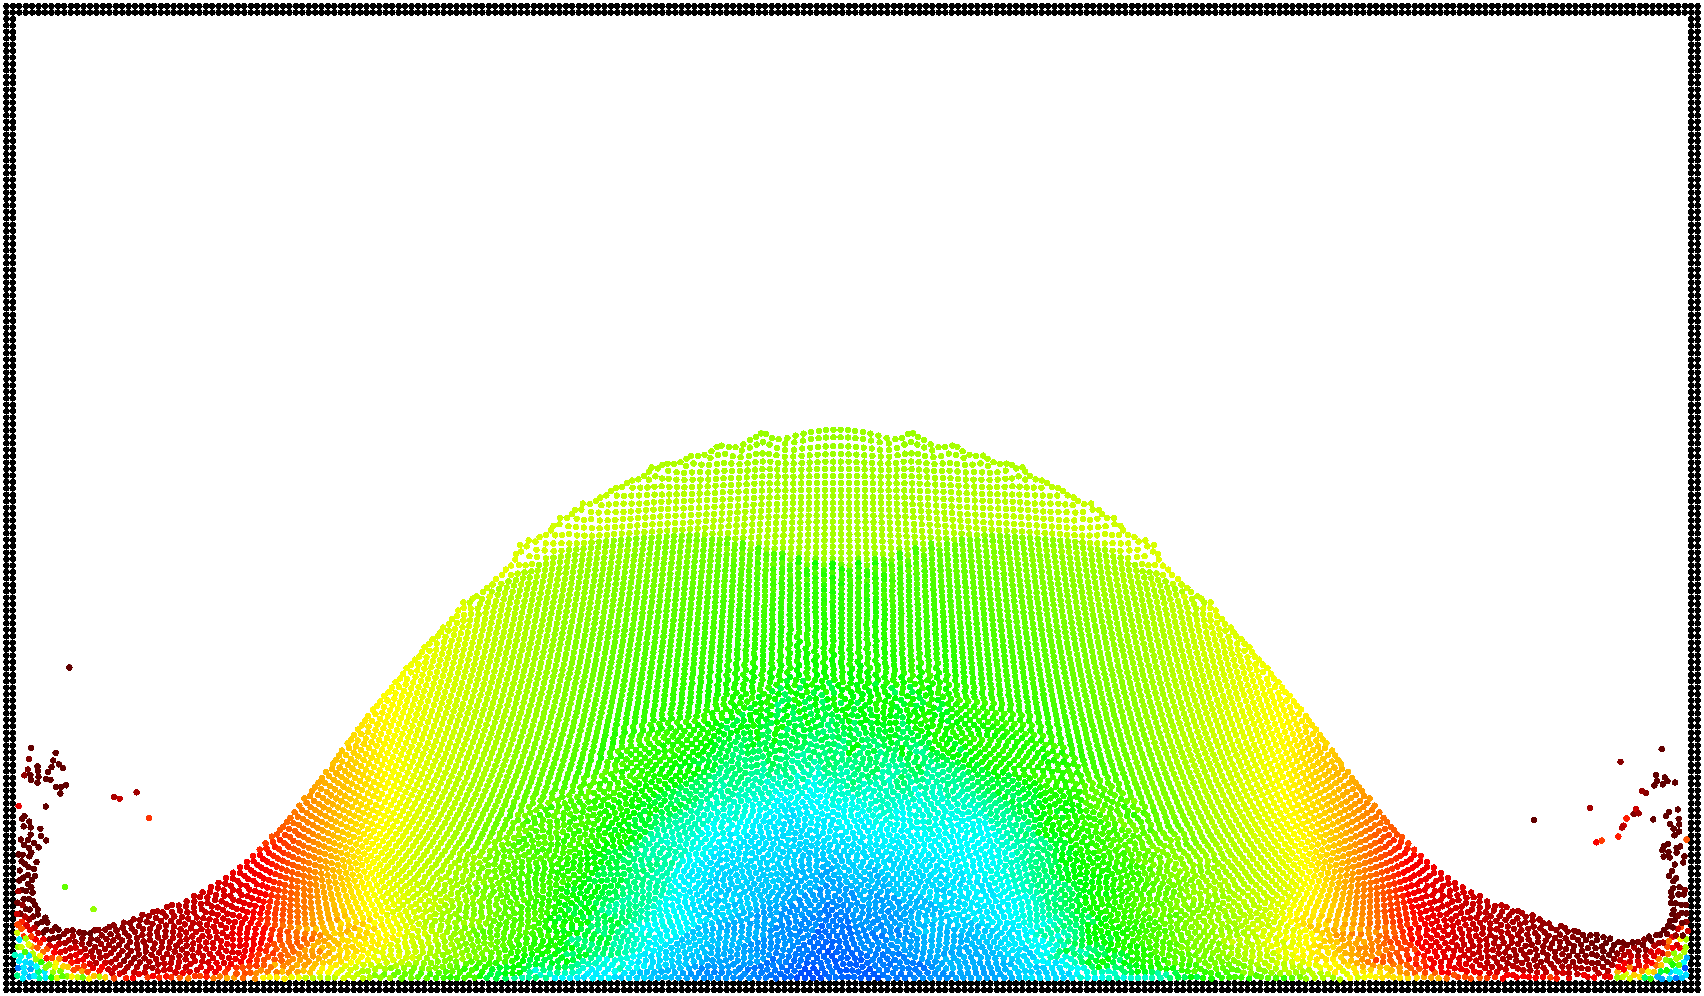
\includegraphics[width=.45\textwidth]{graphics/sim2.png}
	}
	\subfigure[]{
		\centering
		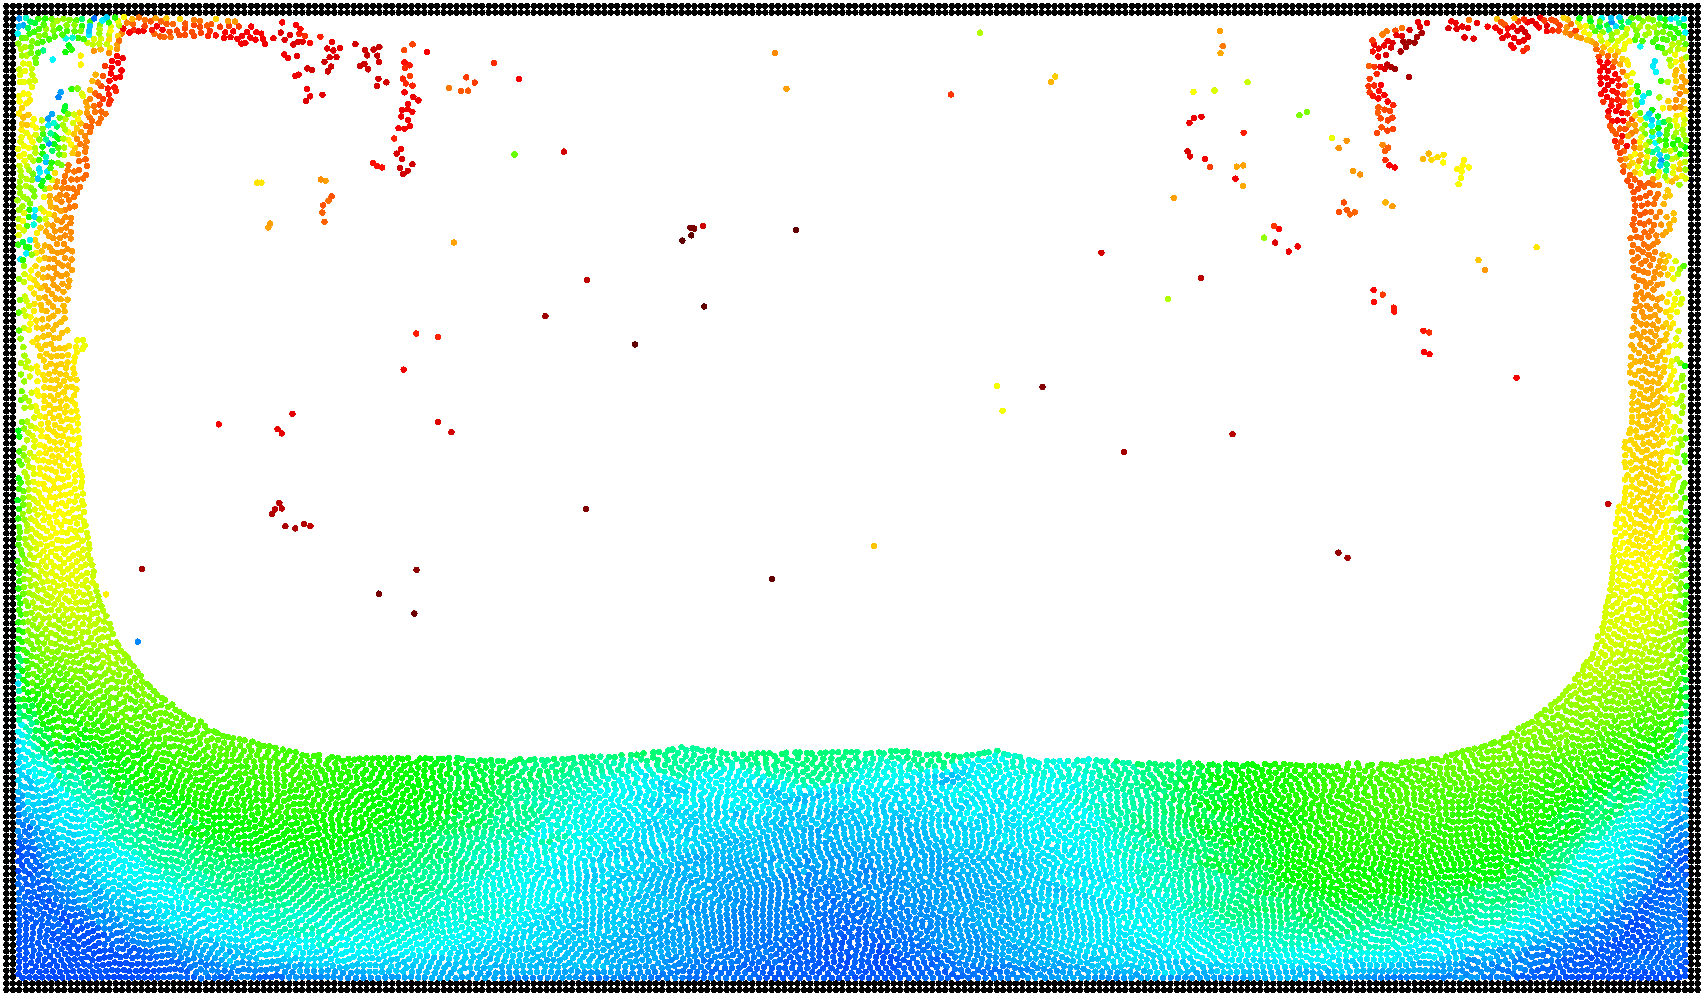
\includegraphics[width=.45\textwidth]{graphics/sim3.png}
	}
	\subfigure[]{
		\centering
		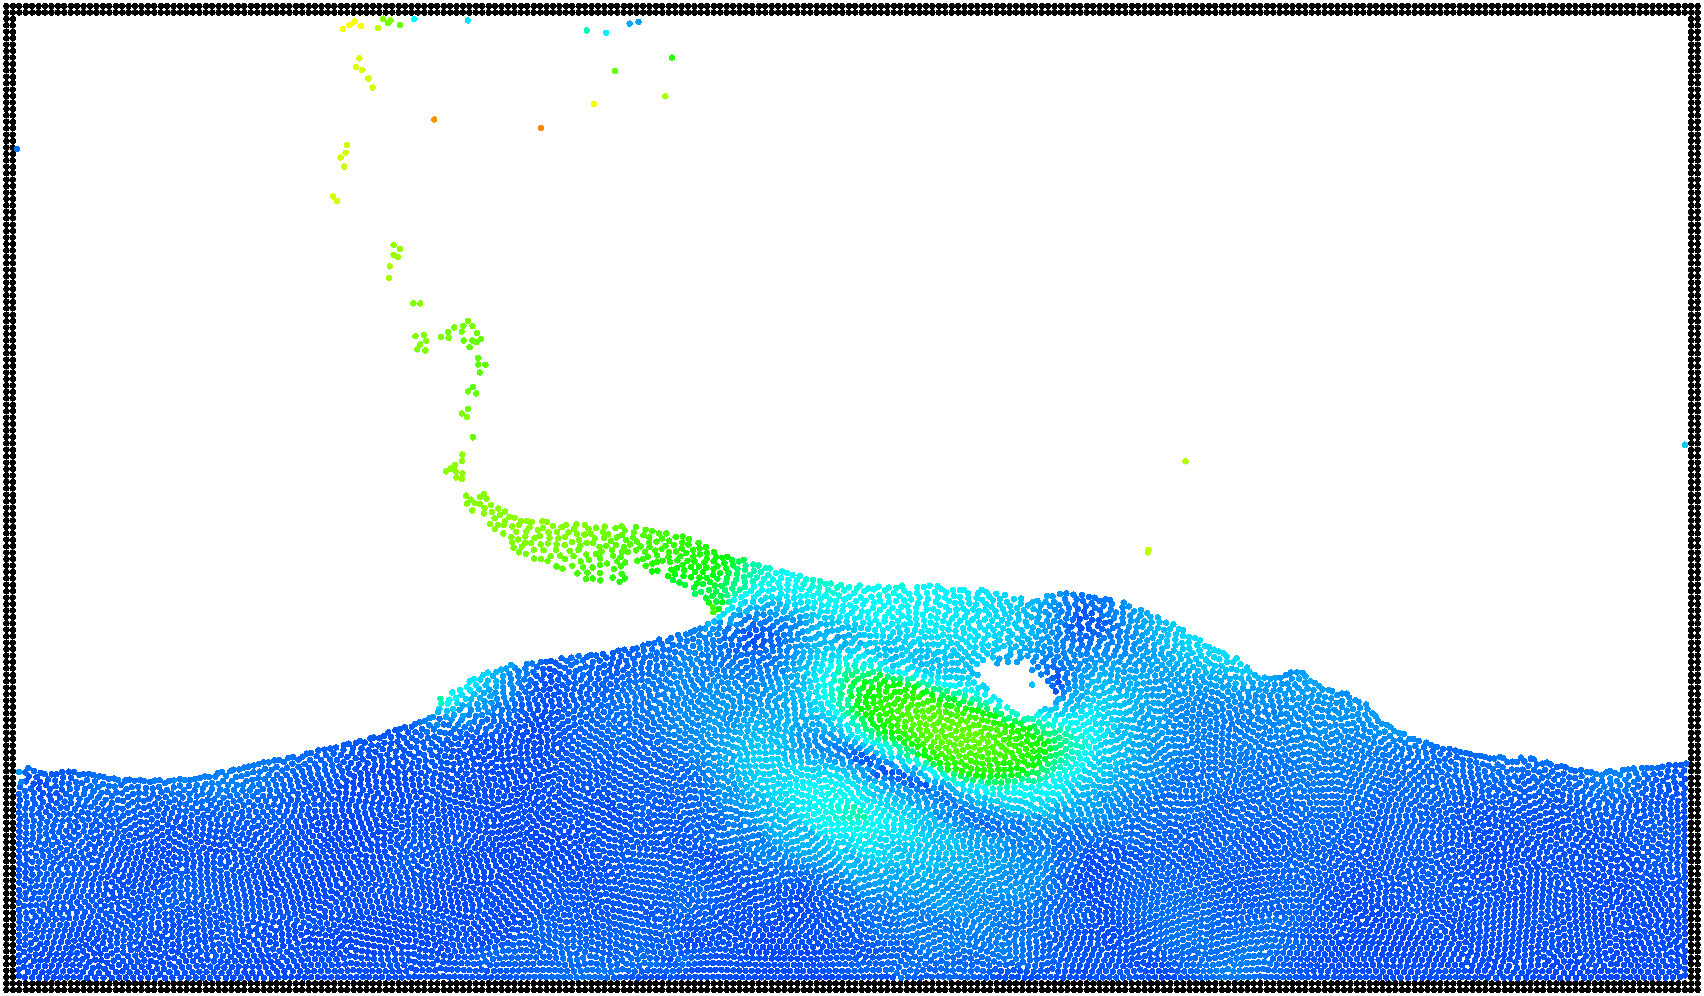
\includegraphics[width=.45\textwidth]{graphics/sim4.png}
	}
	\subfigure[]{
		\centering
		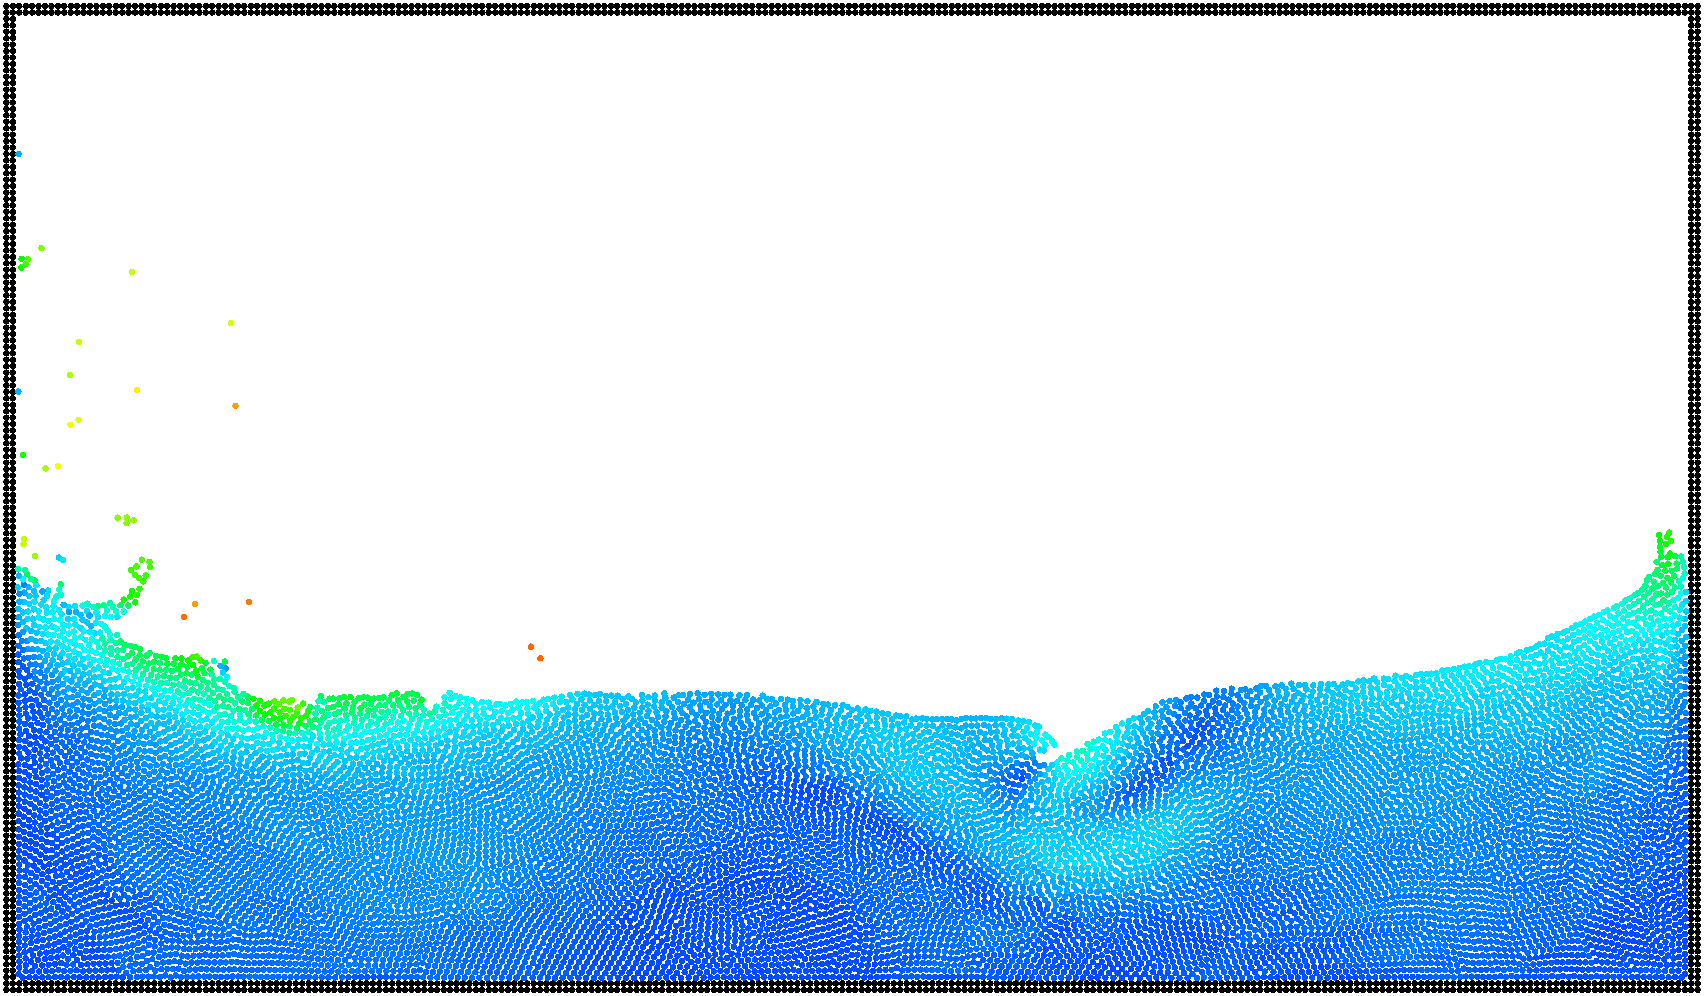
\includegraphics[width=.45\textwidth]{graphics/sim5.png}
	}
	\subfigure[]{
		\centering
		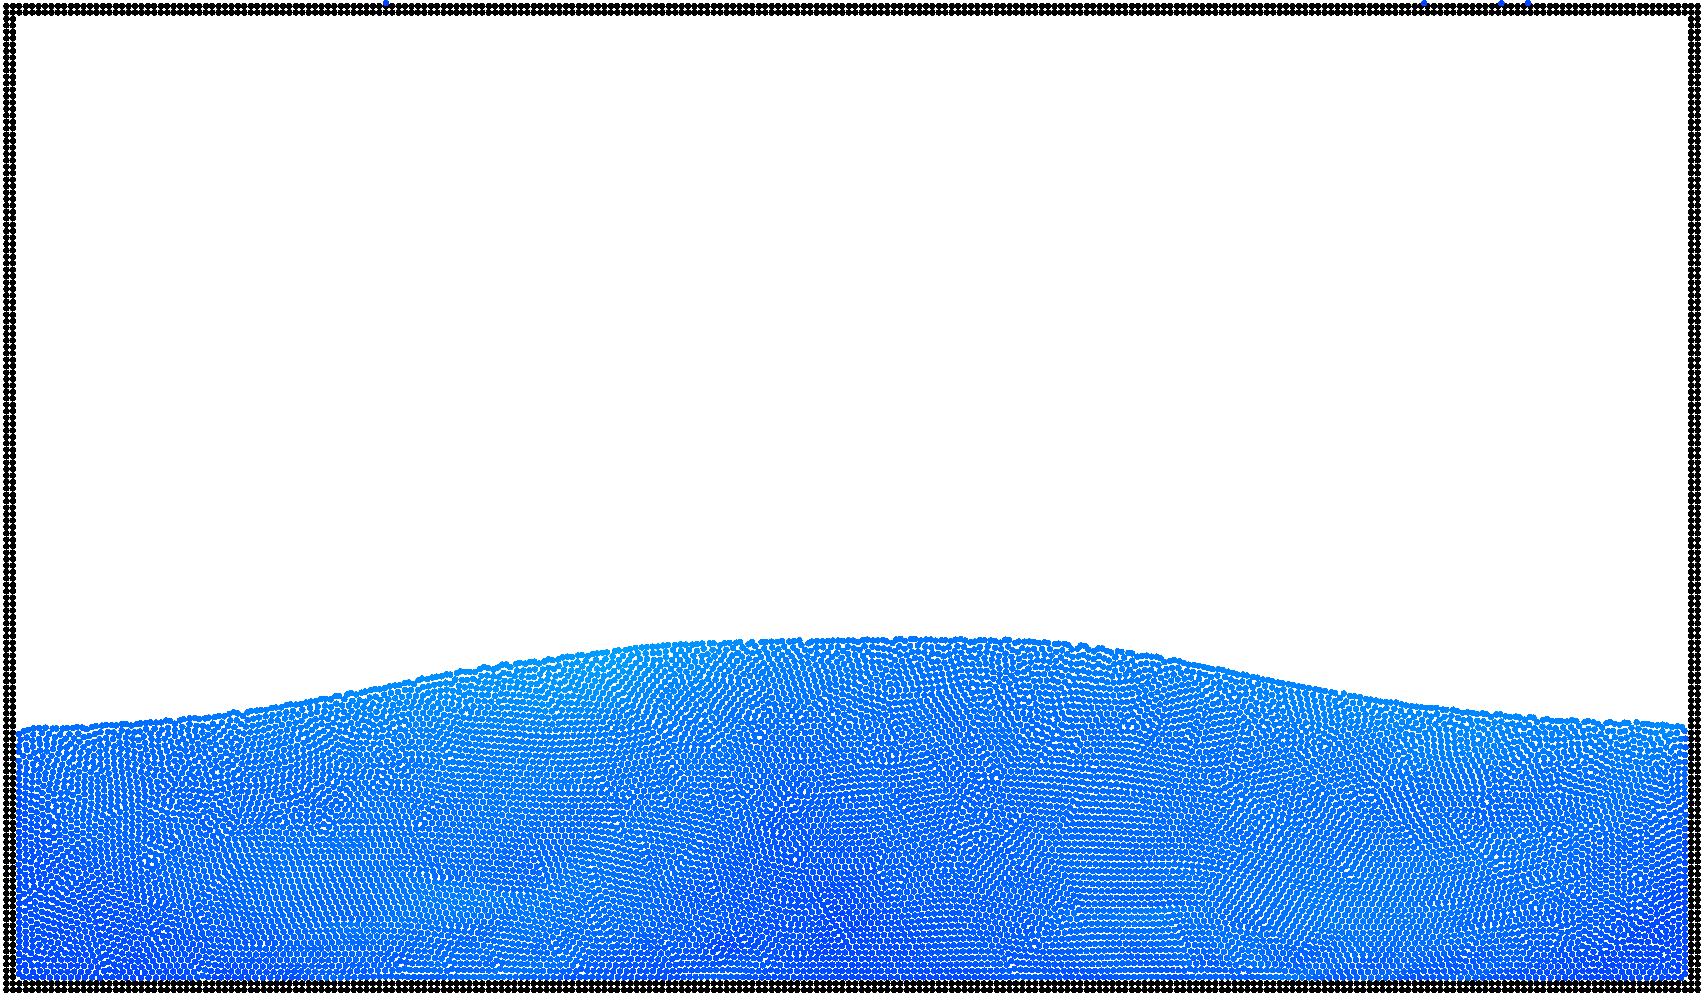
\includegraphics[width=.45\textwidth]{graphics/sim6.png}
	}
	\caption{Ein Fluid, simuliert mit dem implementierten SPH Simulator}
	\label{exampleSimulation}
\end{figure}

Dennoch zeigte sich ein Nachteil dieser Implementierung: Die Parameter müssen szenenabhängig angepasst werden, was einen erheblichen zeitlichen Aufwand erfordert. Zukünftige Arbeiten könnten darauf abzielen, einen Drucklöser zu implementieren, um die Fluiddynamik weiter zu verbessern. Die Einführung eines Drucklösers könnte helfen, den Druck in den Flüssigkeitsbereichen besser zu regulieren und somit die Stabilität der Simulation zu erhöhen.

\nocite{*}
\addcontentsline{toc}{section}{Bibliographie} 
\printbibliography[title={Bibliographie}]

\end{document}